\subsection*{Датчик - нормальный закон}
\addcontentsline{toc}{subsection}{Датчик - нормальный закон}

\textbf{Задание:}\\
Получить нормально распределённую последовательность случайных чисел, используя:
\begin{enumerate}[topsep=0pt,itemsep=-1ex,partopsep=1ex,parsep=1ex]
	\item преобразование Бокса-Мюллера
	\item формулу $Z = \sqrt{\dfrac{12}{n}}\left(\smashoperator[r]{\sum_{i=1}^{n}} x_i - \dfrac{n}{2}\right)$ (частный случай $Z = \smashoperator[r]{\sum_{i=1}^{12}} x_i - 6$)
\end{enumerate}

\textbf{Решение:}\\
\textit{1. Преобразование Бокса-Мюллера}\\

Данное преобразование заключается в замене равномерно распределённых случайных величин на нормально распределённые случайные величины, которые можно найти по следующим формулам:
\begin{ceqn}
	\begin{align*}
		u_1 = \cos(2 \pi \cdot v_1) \sqrt{-2 \cdot \ln(v_2)}\\
		u_2 = \sin(2 \pi \cdot v_1) \sqrt{-2 \cdot \ln(v_2)}
	\end{align*}
\end{ceqn}
То есть на каждом шаге создания нового элемента последовательности нужно сначала сгенерировать два равномерно распределённых случайных числа $v_1$ и $v_2$, а дальше случайно выбрать формулу $u_1$ или $u_2$ для расчёта результирующего элемента последовательности.\\

\newpage
Данный алгоритм был реализован на языке программирования Python. (Рисунок \ref{fig:box_muller_transform_code})
\begin{figure}[h]
	\centering 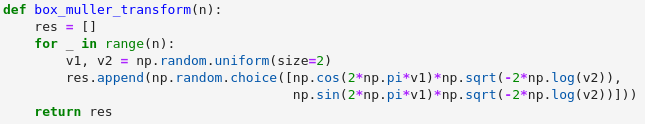
\includegraphics[scale=0.65]{box_muller_transform_code}
	\caption{Реализация преобразования Бокса-Мюллера}
	\label{fig:box_muller_transform_code}
\end{figure}

Была сгенерирована последовательность из 1000 элементов и на основании этого построена гистограмма. (Рисунок \ref{fig:box_muller_transform_result})

\begin{figure}[h]
	\centering 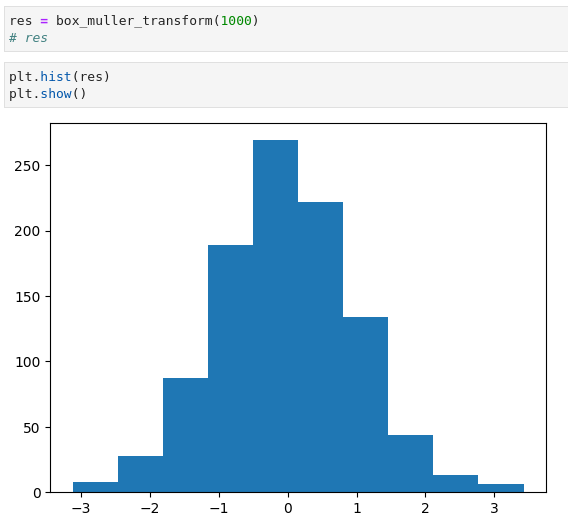
\includegraphics[scale=0.6]{box_muller_transform_result}
	\caption{Результаты применения преобразования Бокса-Мюллера}
	\label{fig:box_muller_transform_result}
\end{figure}

Как можно видеть на получившейся гистограмме, распределение действительно получилось нормальное, то есть алгоритм сработал корректно.

\newpage
Также стоит проверить гипотезу о том, что получившиеся значения распределены нормально. Для этого воспользуемся критерием Колмогорова-Смирнова. (Рисунок \ref{fig:box_muller_transform_test})
\begin{figure}[h]
	\centering 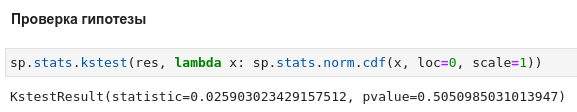
\includegraphics[scale=0.6]{box_muller_transform_test}
	\caption{Результаты теста Колмогорова-Смирнова}
	\label{fig:box_muller_transform_test}
\end{figure}

Значение \textit{p-value} > 0.05, значит мы принимаем гипотезу о том, что данная выборка имеет нормальное распределение.

\vspace{1cm}

\textit{2. Применение центральной предельной теоремы}\\

В данном алгоритме нужно изначально сгенерировать $n$ штук случайных равномерных чисел и дальше воспользоваться формулой, которая вытекает из центральной предельной теоремы:
\begin{ceqn}
	\begin{align*}
		Z = \sqrt{\dfrac{12}{n}}\left(\smashoperator[r]{\sum_{i=1}^{n}} x_i - \dfrac{n}{2}\right)
	\end{align*}
\end{ceqn}

Данный алгоритм был реализован на языке программирования Python. (Рисунок \ref{fig:central_limit_theorem_code})
\begin{figure}[h]
	\centering 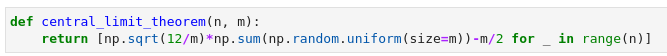
\includegraphics[scale=0.65]{central_limit_theorem_code}
	\caption{Реализация применения центральной предельной теоремы}
	\label{fig:central_limit_theorem_code}
\end{figure}

\newpage
Была сгенерирована последовательность из 1000 элементов и на основании этого построена гистограмма. (Рисунок \ref{fig:central_limit_theorem_result})

\begin{figure}[h]
	\centering 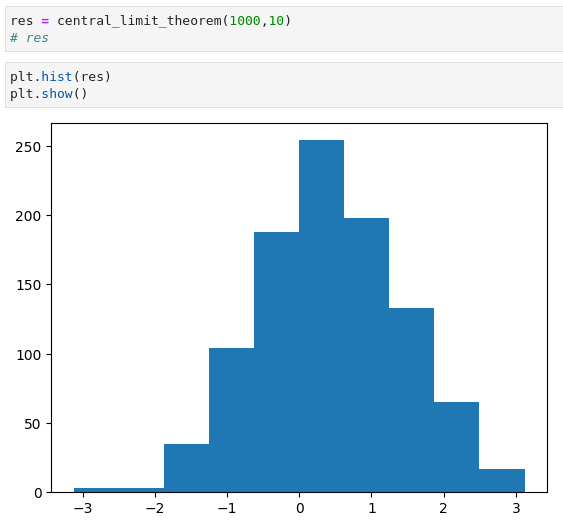
\includegraphics[scale=0.6]{central_limit_theorem_result}
	\caption{Результаты применения центральной предельной теоремы}
	\label{fig:central_limit_theorem_result}
\end{figure}

Как можно видеть на получившейся гистограмме, распределение действительно получилось нормальное, то есть алгоритм сработал корректно.\\

Также стоит проверить гипотезу о том, что получившиеся значения распределены нормально. Для этого воспользуемся критерием Колмогорова-Смирнова. (Рисунок \ref{fig:central_limit_theorem_test})
\begin{figure}[h]
	\centering 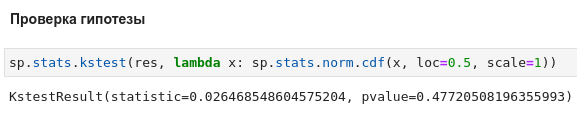
\includegraphics[scale=0.6]{central_limit_theorem_test}
	\caption{Результаты теста Колмогорова-Смирнова}
	\label{fig:central_limit_theorem_test}
\end{figure}

Значение \textit{p-value} > 0.05, значит мы принимаем гипотезу о том, что данная выборка имеет нормальное распределение.